\chapter{The needs of an energy cluster}
\label{ch:background}

\par An Energy Cluster is a group of institutions and businesses working to produce, exchange, and distribute electrical energy. These clusters allow smaller agents in the energy market to cooperate and pool their resources to make their energy infrastructure safer, more efficient, and more profitable. This arrangement allows these entities to get more favorable deals when selling electricity back to the grid. 
\par Energy clusters typically include mid-sized enterprises, smaller individual energy plants, and non-profit organizations, but they can also include larger institutions dedicated solely to generating electricity. 
\par Energy clusters also help to promote the development of renewable energy sources, such as solar, wind, and hydroelectric.

\section{Historical and legal background}

\par Fossil fuels, mainly coal, play a crucial role in Polish energy production. Most energy-producing coal plants were built in the waning decades of the previous century. Since then, renewable energy has been on the constant rise, especially solar technologies, which saw a sudden growth in 2020 thanks to the influx of prosumers - entities simultaneously producing and consuming energy.
\par Five large entities dominate the Polish energy distribution market, each operating in its distribution area. These large distribution network operators (or DNO) are, in order of their size:
\begin{itemize}
  \item Tauron Dystrybucja S.A.
  \item PGE Dystrybucja S.A.
  \item ENERGA-OPERATOR S.A.
  \item Enea S.A.
  \item E.ON Polska S.A. (formerly innogy Polska S.A.)
\end{itemize}
\begin{figure}[htbp]
 \centering
 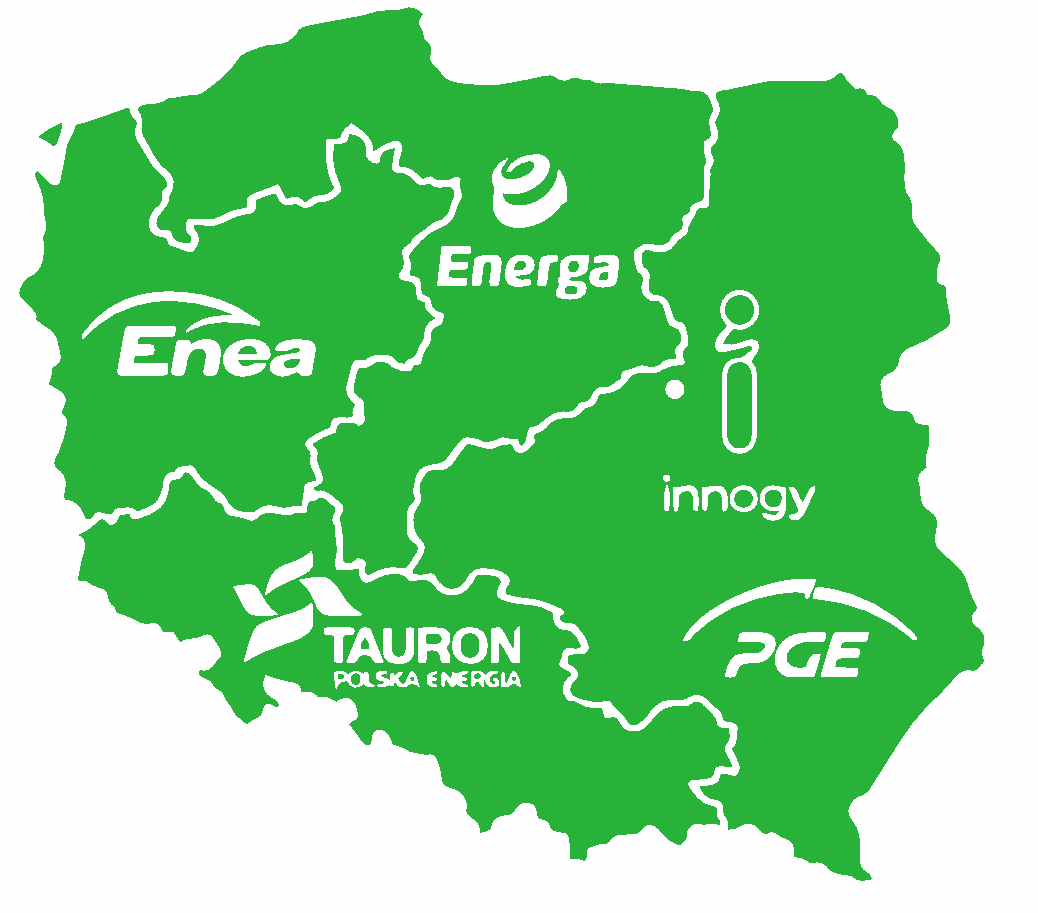
\includegraphics[width=0.5\textwidth]{gfx/EnergyDistributionMap}
 \caption{Distribution Network Operators in Poland}
 \label{fig:chapter02:energydistribution}
\end{figure}
\par Energy Clusters introduce a local alternative to these large enterprises. 
\par The Polish Law defines an energy cluster as "Cywilnoprawne porozumienie, w skład którego mogą wchodzić osoby fizyczne, osoby prawne, jednostki naukowe, instytuty badawcze lub jednostki samorządu terytorialnego, dotyczące wytwarzania i równoważenia zapotrzebowania, dystrybucji lub obrotu energią z odnawialnych źródeł energii lub z innych źródeł lub paliw, w ramach sieci dystrybucyjnej o napięciu znamionowym niższym niż 110 kV, na obszarze działania tego klastra nieprzekraczającym granic jednego powiatu lub 5 gmin. Obszar działania klastra energii ustala się na podstawie miejsc przyłączenia wytwórców i odbiorców energii będących członkami tego klastra." [A Civil law agreement, between natural persons, legal persons, research institutions or local governments, on production, exchange, distribution or turnover of energy from renewable energy sources, or other sources or fuels, as a part of a distribution network with rated voltage lower than 110 kV, and an operational area lower than one county or five municipalities. The energy cluster's operational area is defined, based on the locations of energy producers and consumers, belonging to that energy cluster.]  (art. 2 p. 15a Act on Renewable Energy Sources).
\par These Energy clusters are represented by an Energy Cluster Coordinator, defined by polish law as "Spółdzielnia, stowarzyszenie, fundacja, wskazane w porozumieniu cywilnoprawnym lub dowolny członek klastra energii, powołany w celu reprezentowania klastra" [A cooperative, assocation, foundation, mentioned by a civil law agreement, or any energy cluster member, obligated to represent the cluster] (art. 2 p. 15a Act on Renewable Energy Sources).
\par Energy clusters are thus not an entity onto themself but an accord that defines its participants, operational area, its representative in the form of the coordinator, and its purpose and activities, whether that be production, distribution, sale, or storage of energy. It should also define the rights and responsibilities of every cluster member, the internal organization of the cluster, and how the agreement may be altered or dissolved. 
\par ~
\par One common type of an energy cluster member is the so-called prosumer, a portmanteau of producer and consumer. The RES act defines them as entities buying and producing energy from renewable sources for their own purposes. 

\section{The Energy Cluster infrastructure}

\par The energy cluster members need to agree on the energy delivery method. These entities can exchange energy by using either: 
\begin{itemize}
  \item existing infrastructure
  \item their private infrastructure
  \item a hybrid model consisting of the previous options
  \item Enea S.A.
  \item E.ON Polska S.A. (formerly innogy Polska S.A.)
\end{itemize}
\par The most economical and popular option is to use the public energy grid. In such cases, the energy cluster coordinator has to apply with the appropriate DNO for access to the infrastructure, and the DNO is obligated to, whenever possible, connect every applying entity to the existing grid without prioritizing any other entity.
\par The less common option is to use a private energy grid explicitly made for the energy cluster. This method comes with responsibilities similar to those imposed on more traditional entities outside the energy cluster and much higher costs than using the public grid. It can, however, be economically sound in the case of a few large energy producers close to one another.

\section{The Energy Cluster organization}

\par In order to establish a functioning energy cluster, its members should:
\begin{enumerate}
  \item Define a name and location for the cluster
  \item List all of the cluster members
  \item Name the cluster coordinator and establish the functions and responsibilities of the cluster members
  \item Describe the infrastructure used by the cluster to produce, transmit and store energy
  \item Measure the current energy needs of every member, and find out how much of it is satisfied by producers inside the cluster
  \item Measure how much energy is currently satisfied by RES and how much will be satisfied by them in 10 years.
  \item Measure how much
\end{enumerate}
~ Is this plagiarism?

\section{Members of an energy cluster}

\par Various entities compose an energy cluster, some of which produce or consume energy, and others handle organizational matters. 
\par Local governments are frequently initiators of such enterprises, especially given their benefits to the local economy and government funding provided for energy cluster development. It can mediate between competing cluster members or help procure necessary funding faster and more efficiently.
\par Some of the most vital members of energy clusters are local businesses. Their membership is mutually beneficial since while energy clusters can help their development, such enterprises provide the necessary funding and experience to build the clusters network faster.
\par ~Producers and prosuments?
\par Every energy cluster needs to choose, amongst its members, a coordinator to represent the cluster. It is usually a private company operating in the energy distribution market with the necessary funds and permits to produce and distribute energy. It can apply for any further permits needed in the future and take loans in the name of the cluster. Sometimes that company acts exclusively as an energy cluster coordinator, efficiently managing the entire system.
\par The coordinator can also be an association of natural persons making up the energy cluster, a foundation comprising both natural and legal persons, a cooperative, or a company. It cannot be a legal person, such as a partnership or a homeowner association.
